\documentclass[12pt,letterpaper]{article}
\usepackage[latin1]{inputenc}
\usepackage{amsmath}
\usepackage{amsfonts}
\usepackage{amssymb}

% the above packages are the "base"

\usepackage{graphicx}
\graphicspath{{../figs/}} % set the location of your figures

\usepackage{hyperref} % enable links within pdf
\hypersetup{colorlinks = true, linkcolor = black, urlcolor = blue}


\usepackage{bm}
\usepackage{xcolor}



\usepackage{fancyvrb}

\usepackage{listings} % to typeset in R format
\xdefinecolor{gray}{rgb}{0.4,0.4,0.4}
\xdefinecolor{blue}{RGB}{58,95,205}% R's royalblue3; #3A5FCD
\lstset{% setup listings
	language=R,% set programming language
	basicstyle=\ttfamily\small,% basic font style
	keywordstyle=\color{blue},% keyword style
	commentstyle=\color{gray},% comment style
	numbers=left,% display line numbers on the left side
	numberstyle=\scriptsize,% use small line numbers
	numbersep=10pt,% space between line numbers and code
	tabsize=3,% sizes of tabs
	showstringspaces=false,% do not replace spaces in strings by a certain character
	captionpos=b,% positioning of the caption below
	breaklines=true,% automatic line breaking
	escapeinside={(*}{*)},% escaping to LaTeX
	fancyvrb=true,% verbatim code is typset by listings
	extendedchars=false,% prohibit extended chars (chars of codes 128--255)
%	literate={"}{{\texttt{"}}}1{<-}{{$\bm\leftarrow$}}1{<<-}{{$\bm\twoheadleftarrow$}}1
%	{~}{{$\bm\sim$}}1{<=}{{$\bm\le$}}1{>=}{{$\bm\ge$}}1{!=}{{$\bm\neq$}}1{^}{{$^{\bm\wedge}$}}1,% item to replace, text, length of chars
	alsoletter={.<-},% becomes a letter
	alsoother={$},% becomes other
	otherkeywords={!=, ~, $, \&, \%/\%, \%*\%, \%\%, <-, <<-, /},% other keywords
	deletekeywords={c}% remove keywords
}


\setcounter{secnumdepth}{0}  % don't number sections (stars not needed)


%\author{Mark Novak}
\title{Coding best practices}

\begin{document}
\maketitle

\tableofcontents

\pagebreak

The reality is that for any non-trivial task, most of your time will be spent de-bugging your code, not
writing it.  There are two over-arching principles that will, when practiced, greatly increase your
efficiency:  writing \emph{modular} code and writing \emph{clean} code.  In class we'll discuss
modularity first (it relates to the \emph{project mindset} referred to in the context of \texttt{git}) and will
then talk about code-writing best practices (styles guides).

\section{Principle of Modularity}
If your experience learning to code as been anything like mine then, either when you first started coding or when you wrote homework assignments for Stats class, the code you created for a given project probably consisted of one long giant file.  If you learned to use \texttt{Markdown} or \texttt{Sweave}, that code probably had some number of sections within it, just like you might write a paper or thesis chapter (Intro, Methods, Results).

That'll work fine for small (tiny) projects or homework reports, but probably not for anything the size of a paper or thesis chapter that contains some combination or subset of data, analyses (whether statistical or non-statistical modeling), and data- or results visualization.

Thus, as alluded to in \nameref{projectfolder}, you should give your project a useful structure:

Your \texttt{data} folder should contain all the data you need for the project.  Most of the time, this will include both the \emph{original} unedited raw data files (regardless of their format) as well as \emph{derived} data files (that you have used code to produce).  No files should be duplicates or derived copies of each other (see Fig. \ref{fig:datafilenames}); remember: versions will be tracked by \texttt{git}.

Your \texttt{code} folder contains your various script files.  For anything but the smallest projects there should be multiple files that contain scripts for performing different tasks.  For example, you might have:

\begin{tabular}{p{0.2\linewidth}p{0.8\linewidth}}
	\texttt{data\_prep.R} & Script that pulls in the original data, pre-processes them (rearranges, correct errors, standardizes names, splits up or merges different data sets), and spits them back out in a ``clean'' format needed by your subsequent analyses \\
	\texttt{my\_functions.R} & Script containing the functions you have self-defined to perform your analyses \\
	\texttt{analysis.R} & Script that sucsk in your ``clean'' data, performs your analyses (using built-in, self-defined and package functions), makes some quick-and-dirty figures along the way, and exports the results to \texttt{output} \\
	\texttt{final\_figs.R} & Script that sucks in the results of the analyses to produce the final figures (or tables) for your manuscript\\

\end{tabular}

In general, you don't want any file to become unwieldy.  Thus you will likely have multiple scripts within each of the above categories (e.g., one for each of several different data set types, one for each of several different analyses or analysis steps, or one for each of several different self-defined functions) -- each appropriately named (see \nameref{codestyleguide}).  If you end up with a whole lot of scripts to perform an analysis from start to finish, then you may want one additional \texttt{RunMe.R} script that sources each of the other scripts in the appropriate order.


The key utilities of separating out everything as specified above are (1) \emph{readability} and (2) \emph{unit-testing}.    Readability means that it's easy for anyone (including you in 1 years time) to figure out where things are being pulled from and where they're going, and no individual script is overwhelming to look through.  The idea behind unit-testing is to write independent tests for the smallest units of your code.  For example, whenever you write a function, you also write an associated small piece of code that tests it (before the function is used in your primary analysis). That way, whenever you modify your code or function(s), it's easy to ensure that everything is still returning the correct output.



\begin{figure}
	\centering
	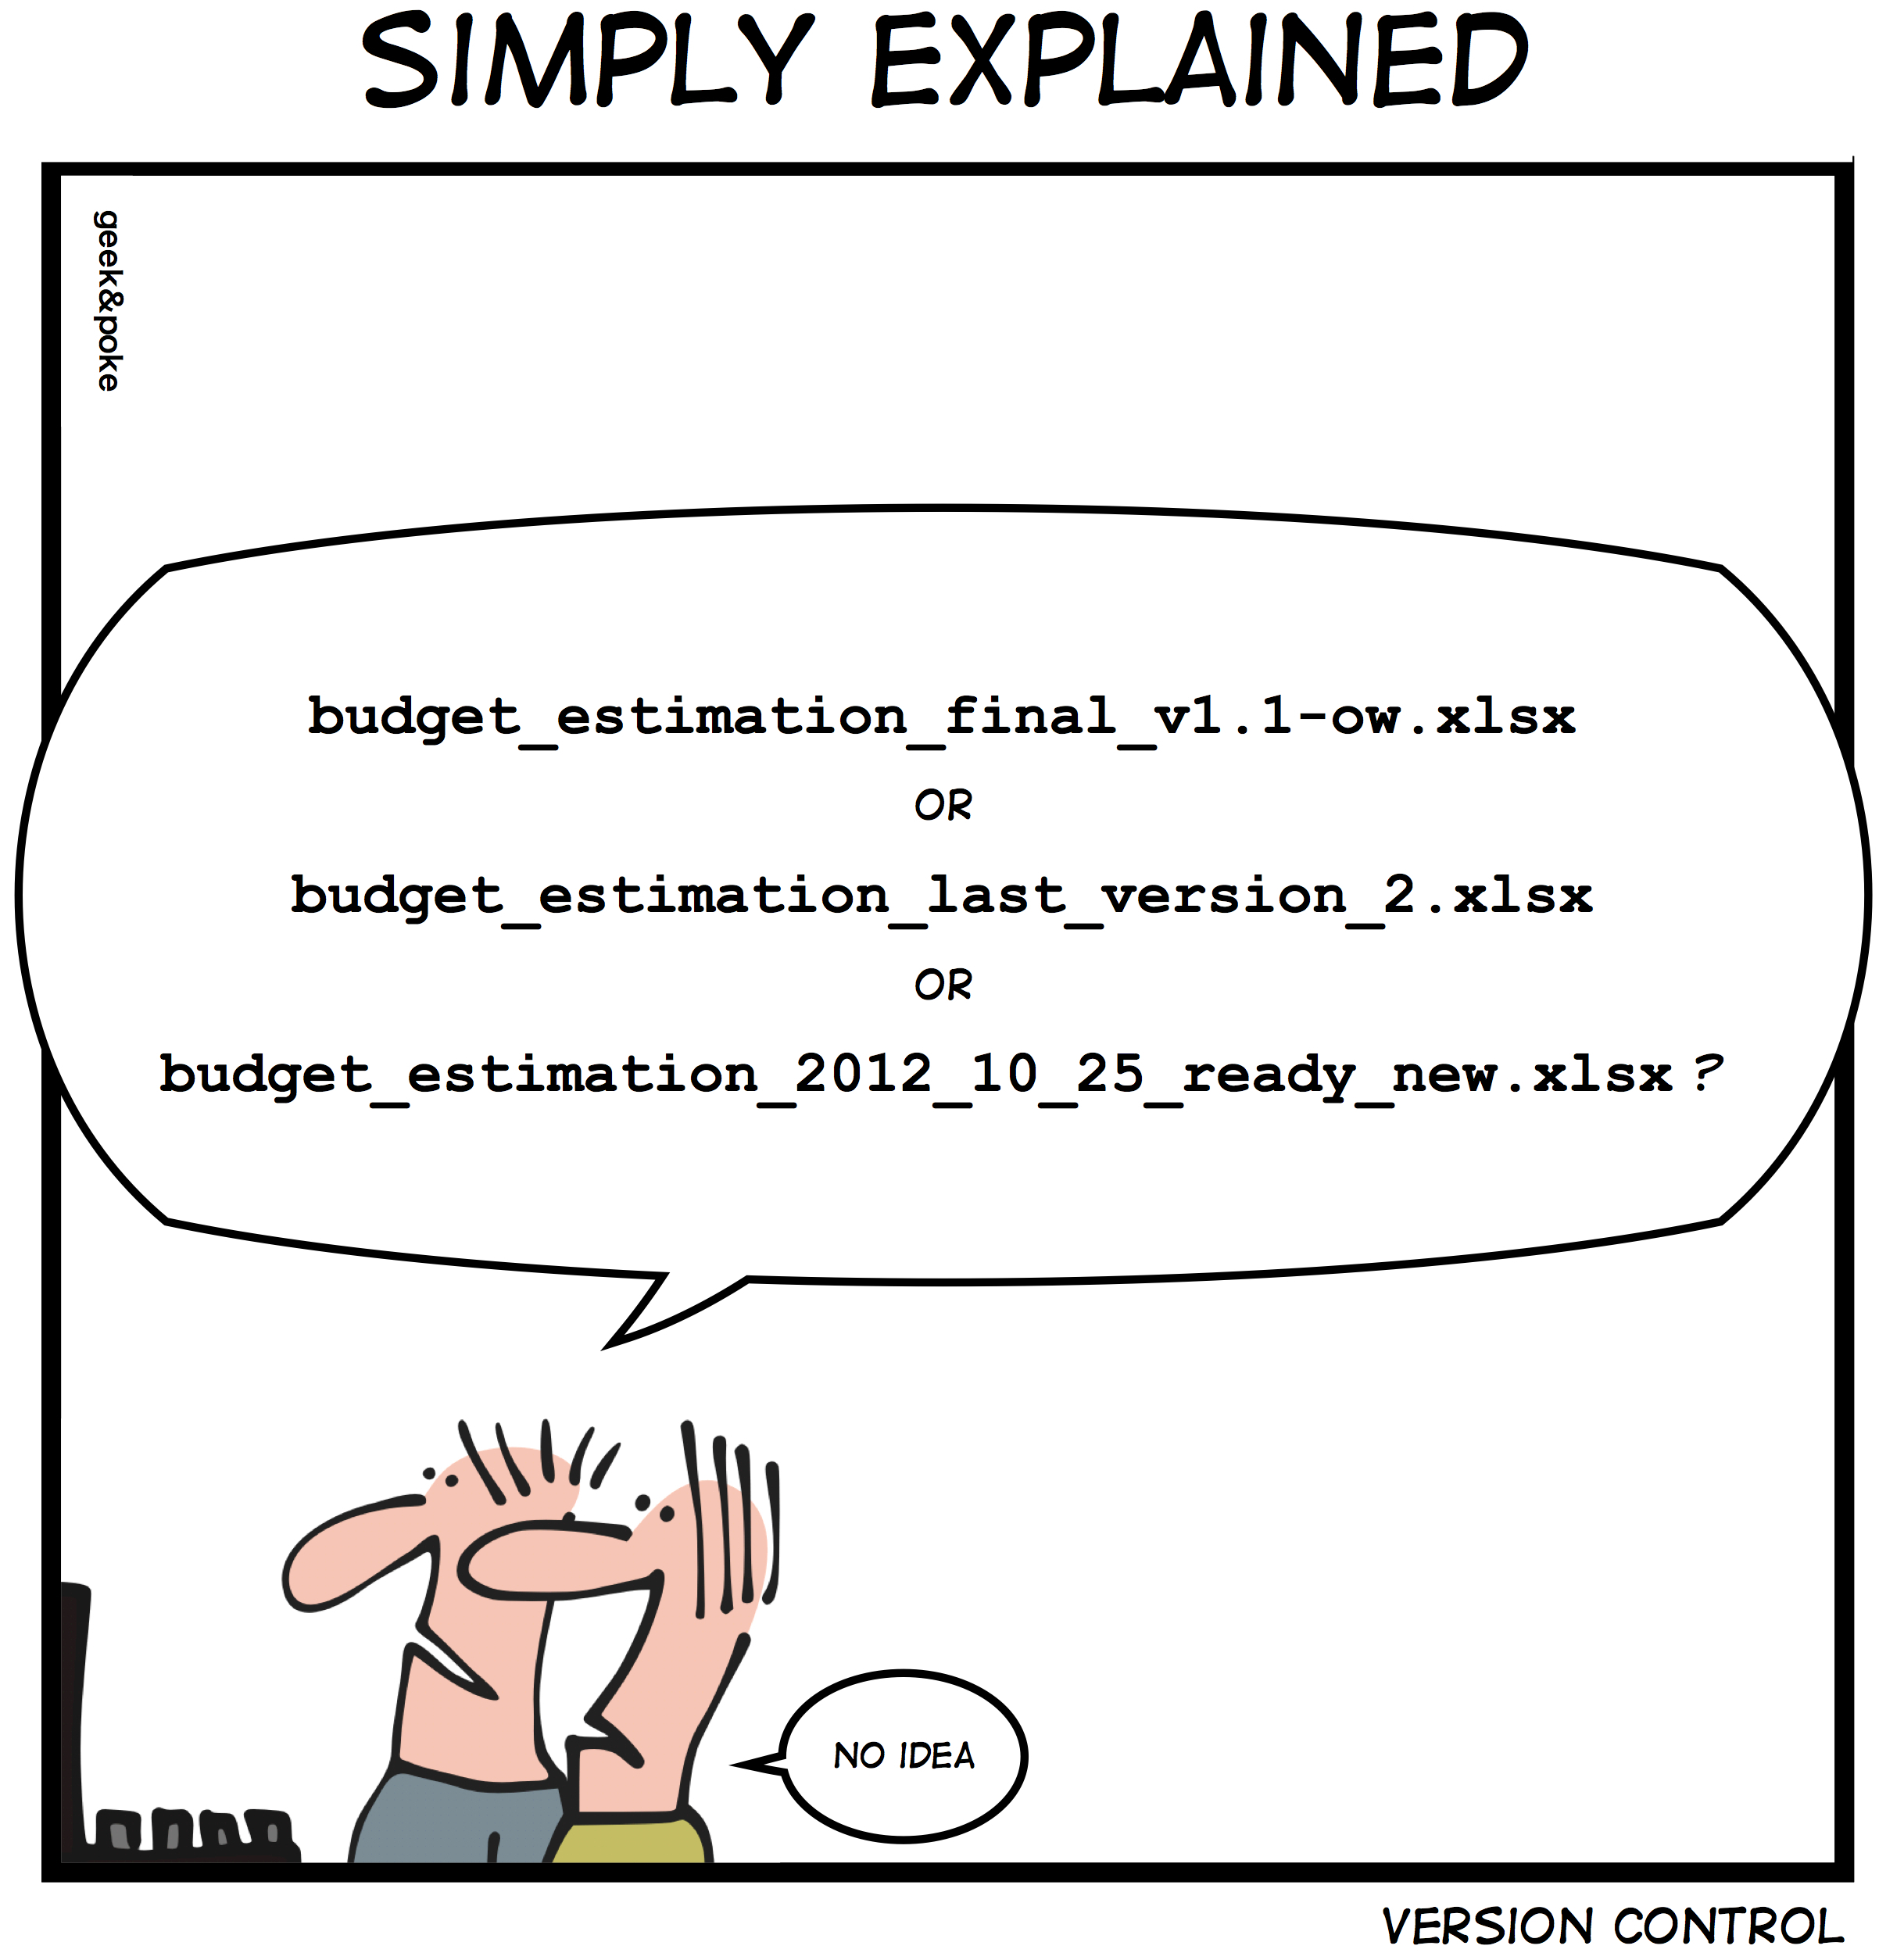
\includegraphics[width=0.8\linewidth]{datafilenames.jpg}
	\caption{Never again should your data files look like this!}
	\label{fig:datafilenames}
\end{figure}

\subsection{Working directory and directory access}
In order to employ the principle of modularity you need to know how to navigate between your various folders and scripts.  Within a project, for example, you have a choice between using the repository folder as your working directory or setting your working directory to be the directory in which you have saved your scripts (e.g., your RunMe script). Your scripts will therefore need to access data and source scripts that are located in other folders.  You want to set these locations as generically as possible (so that you can move your entire project to a different location without destroying the workflow, for example).  You never want to set the working directory more than once, or hard-write the locations of your data or other scripts within a given script.

You can do this by specifying locations relationally using `\texttt{/.../file.R}', for example. Each repetition of `\texttt{/.../}' will move you up one level in the folder structure.   For example, assuming your working directory is the \texttt{code} directory, rather than specifying the location of your data as

\texttt{read.csv(file=`C://MyDocuments/Git/MyProject/data/data.csv')}

you should instead use

\texttt{read.csv(file=`.../data/data.csv')}.

The latter takes you up one level (out of \texttt{code} into your general \texttt{repository} folder) then into the \texttt{data} folder and to your data file.  To pull in scripts, use

\texttt{source(file=`my\_functions.R')}

(assuming your working directory is the \texttt{code} directory).

\textbf{Note:} Macs (Unix) and Windows (Dos) use forwardslashes and backslashes differently.  Macs use `\texttt{/.../.../file.R}' (forwardslashes) while Windows use `\texttt{\textbackslash...\textbackslash...\textbackslash file.R}' (backslashes).


\section{Code style guides} \label{codestyleguide}
There are a lot of summarized sets of recommended best-practices for coding in general and for \texttt{R} as well.  These includes aspects relating to object naming conventions (for filenames, function names, and variable names), syntax and grammar (spacing, indentation, etc.), and code structure.  I won't repeat everything here, but we will go over and discuss the big ones in class.  For our course, the \textbf{required reading} is:

\url{https://google.github.io/styleguide/Rguide.xml}

Other guides that are well worth reading for some additional suggestions and explanations are:

\url{https://www.r-bloggers.com/r-code-best-practices/}

and

\url{http://adv-r.had.co.nz/Style.html}


\section{Within-script organization}
In additional the best practices in the naming of objects and the syntax of your code, there's also an important aspect of within-code organization. Your code should consist of the following sections, each visually separated from the others:

\begin{enumerate}

	\item Start each file with a preface that describes what it contains and how it fits into the project. You might also want to include who wrote it and when.

	\item Load all required packages

	\item Source required scripts (e.g., \texttt{my\_functions.R})

	\item Load (or source) required data (or \texttt{data\_prep.R} scripts)

	\item Section(s) for major parts of your analyses

	\item Export results section(s)

\end{enumerate}
The last two may consist of just two sections or may have export parts immediately following an analysis.  Wherever possible and appropriate, clear your workspace (\texttt{rm(list=ls())}).  For example, you'd most definitely do this at the top of your \texttt{RunMe.R} script and perhaps to at the top of your \texttt{analysis.R} script (since your ``cleaned'' data was saved and can be reloaded, leaving all the temporary variables unnecessary), but you wouldn't put \texttt{rm(list=ls())} at the head of your \texttt{my\_functions.R} script.

Thus a script file might look as follows:

\noindent\rule{12cm}{0.4pt}
\begin{lstlisting}[language=R]
########################################################
# simulateLV.R
# Simulates the dynamics of a predator and prey population according to the Lotka-Volterra model.
# The data produced will subsequently be used to test the performance of several population dynamic model-fitting routines.
########################################################
rm(list=ls()) # clear workspace

##############################
# Load librairies
##############################
library(deSolve)

##############################
# Source files
##############################
# None needed

##############################
# Define model
##############################
LVmod <- function(Time, State, Pars) {
	with(as.list(c(State, Pars)), {
		Ingestion    <- rIng  * Prey * Predator
		GrowthPrey   <- rGrow * Prey * (1 - Prey/K)
		MortPredator <- rMort * Predator

		dPrey        <- GrowthPrey - Ingestion
		dPredator    <- Ingestion * assEff - MortPredator

		return(list(c(dPrey, dPredator)))
		})
	}

##############################
# Define parameters
##############################
pars <- c( rIng   = 0.2,    # /day, rate of ingestion
	      rGrow  = 1.0,    # /day, prey growth rate
	      rMort  = 0.2 ,   # /day, predator mortality
	      assEff = 0.5,    # assimilation efficiency
	      K      = 10)     # mmol/m3, carrying capacity

##############################
# Simulate model
##############################
yini  <- c(Prey = 1, Predator = 2)
times <- seq(0, 200, by = 1)
out   <- ode(yini, times, LVmod, pars)
summary(out)

##############################
# Plot and export data
##############################
plot(out)
write.csv(out, file=`.../output/LV_out.csv')

##########################################################
\end{lstlisting}
\noindent\rule{12cm}{0.4pt}

When defining a function, you should provide additional information that describes what the function does (in general terms), what inputs it takes, and what output it returns.  After the function is defined it's worth adding a test case (commented out).  [Note: some would separate out test cases, leaving only the function definition in its own script.]  For example:

\noindent\rule{12cm}{0.4pt}
\begin{lstlisting}[language=R]
########################################################
# Function to add stochastic noise to a time-series of population sizes.
########################################################
# Input:
#	x -- a time series of population sizes (vector)
#	error_model -- gaussian (currently implemented model, default)
# 	sd -- the standard deviation of gaussian errors (default=0)
# Returns:
#	Vector of length equal to the input vector of time series

add_error <- function(x, error_model=`gaussian', sd=0){
	error_model <- match.arg(error_model)
	if(error_model==`gaussian'){
		out <- x + rnorm(length(x), sd)
	}else{
		out <- x
		warning(``Original time series returned'')
	}
	return(out)
}

# Test:
# source(`simulateLV.R')
# new <- add.error(out, sd=1)
# par(mfrow=c(1,2))
#	plot(out)
#	plot(new)
\end{lstlisting}
\noindent\rule{12cm}{0.4pt}


\section{When writing code, though shalt not...}

\begin{itemize}
\item Copy-paste-edit (i.e. reuse and modify) the same code to repeatedly apply it to different subsets of data, etc..  Instead, you will convert your code to function(s) that can be applied to these data subsets
\item Use \texttt{attach()} and \texttt{detach()} on your data.  Instead, be explicit in naming and accessing data.frame columns.
\item Repeatedly reset your working directory.  Instead, use relational sourcing.
\item Save your \textsf{R} workspace for later reuse.  Instead, use \texttt{rm(list=ls())} wherever possible and appropriate.
\item create large tables by hand. If you find yourself having to export large tables a lot, learn \LaTeX and export them instead
\end{itemize}


\end{document}
